\documentclass[12pt]{article}

\usepackage[margin=1in]{geometry}
\usepackage{amsmath}
\usepackage{graphicx}
\usepackage{float}
\usepackage{caption}
\usepackage{enumitem}
\graphicspath{{../fig/}{fig/}}

\title{Archived Analysis: Household Inflation Burden}
\author{Erwan Gautier and J\'er\'emi Montorn\`es}
\date{\today}

\begin{document}
\maketitle

This standalone copy preserves the inflation-burden analysis, which has been restored to the main
manuscript with an explicit interpretation caveat. Net household income is used both to assign
income quintiles and as the denominator of the burden measure. The resulting Q1--Q5 gradient can
therefore partly reflect a mechanical expenditure-to-income gradient rather than heterogeneous
inflation exposure. Before interpreting the gradient as an inflation-exposure effect, the analysis
should:
\begin{enumerate}[nosep]
  \item decompose the gap into heterogeneous inflation and heterogeneous expenditure-to-income ratios;
  \item report both means and medians;
  \item test alternative winsorization thresholds;
  \item rank households using equivalised income; and
  \item calculate the burden under a common inflation rate to isolate the mechanical denominator channel.
\end{enumerate}

\section{Inflation Burden}

Our indicators measure differences in inflation exposure across household groups, but they do
not directly express the cost of inflation relative to household resources. We therefore construct
the burden from HBS microdata rather than combining group-level inflation with an external aggregate
consumption-to-income ratio. For household $i$ in country $c$, let $X_{ic}$ denote consumption
expenditure on the non-rent products matched to HICP, $Y_{ic}$ net household income, and
$\bar{\pi}_{ic,y}$ the household's average annual inflation rate in year $y$, computed with the
RAS-calibrated weights used in the main manuscript. The raw household-level burden is
\begin{equation}
\mathcal{B}^{\mathrm{raw}}_{ic,y}=\bar{\pi}_{ic,y}\frac{X_{ic}}{Y_{ic}}.
\end{equation}
Because $\bar{\pi}_{ic,y}$ is measured in percent, $\mathcal{B}^{\mathrm{raw}}_{ic,y}$ is measured in
points of net income. The indicator allows both individual inflation exposure and the
consumption-to-income ratio to vary across households. The expenditure numerator and inflation
index cover the same matched non-rent products. This fixed-resource exposure indicator is not
compensating variation: it holds 2020 expenditure and income fixed and allows neither substitution
nor income adjustment.

Very small reported incomes can generate mechanically extreme expenditure-to-income ratios. We
therefore winsorize $100X_{ic}/Y_{ic}$ at the survey-weighted 99th percentile within each country,
while retaining the underlying household inflation rate. Denoting the resulting ratio by
$\widetilde{\kappa}_{ic}$, the burden used in the estimates and its aggregation for national income
quintile $q$ are
\begin{equation}
\mathcal{B}_{ic,y}=\bar{\pi}_{ic,y}\frac{\widetilde{\kappa}_{ic}}{100},
\qquad
\mathcal{B}_{q,y}=\frac{\sum_{c}\sum_{i\in q(c)}a_{ic}\mathcal{B}_{ic,y}}
{\sum_{c}\sum_{i\in q(c)}a_{ic}}.
\end{equation}
Here $a_{ic}$ is the HBS survey weight, and $q(c)$ indicates that total-net-income quintiles are
defined separately within each country before households are pooled. The survey weights expand the
microdata to national household populations and therefore determine the euro-area aggregation.
The 2020 HBS basket, income, and expenditure observations are held fixed, while household-specific
inflation is calculated for 2021--2023. For each household-year, the inflation rate is computed over
the matched non-rent expenditure categories and the HBS--HICP product weights are renormalized to
one. We impose no minimum matched-expenditure threshold.

Higher-income households also generally have greater capacity to absorb a price shock by reducing
discretionary expenditure or substituting toward cheaper varieties. The main manuscript's appendix
documents the corresponding difference in basket composition.

Figure~\ref{fig:archived-inflation-burden} uses household indices and matched non-rent expenditure.
The first quintile faces a burden of 2.5 percent of net income in 2021, 8.7 percent in 2022, and
4.8 percent in 2023, compared with 1.5, 4.7, and 3.0 percent for the fifth quintile. The Q1--Q5 gap
is 1.0, 4.0, and 1.8 points, respectively, calculated before rounding. The income and expenditure
filters retain positive-income households; national quintiles are assigned before these
burden-specific exclusions.

\begin{figure}[H]
\centering
\caption{Household-level inflation burden in the euro area, by income quintile (in \% of net income)}
\label{fig:archived-inflation-burden}
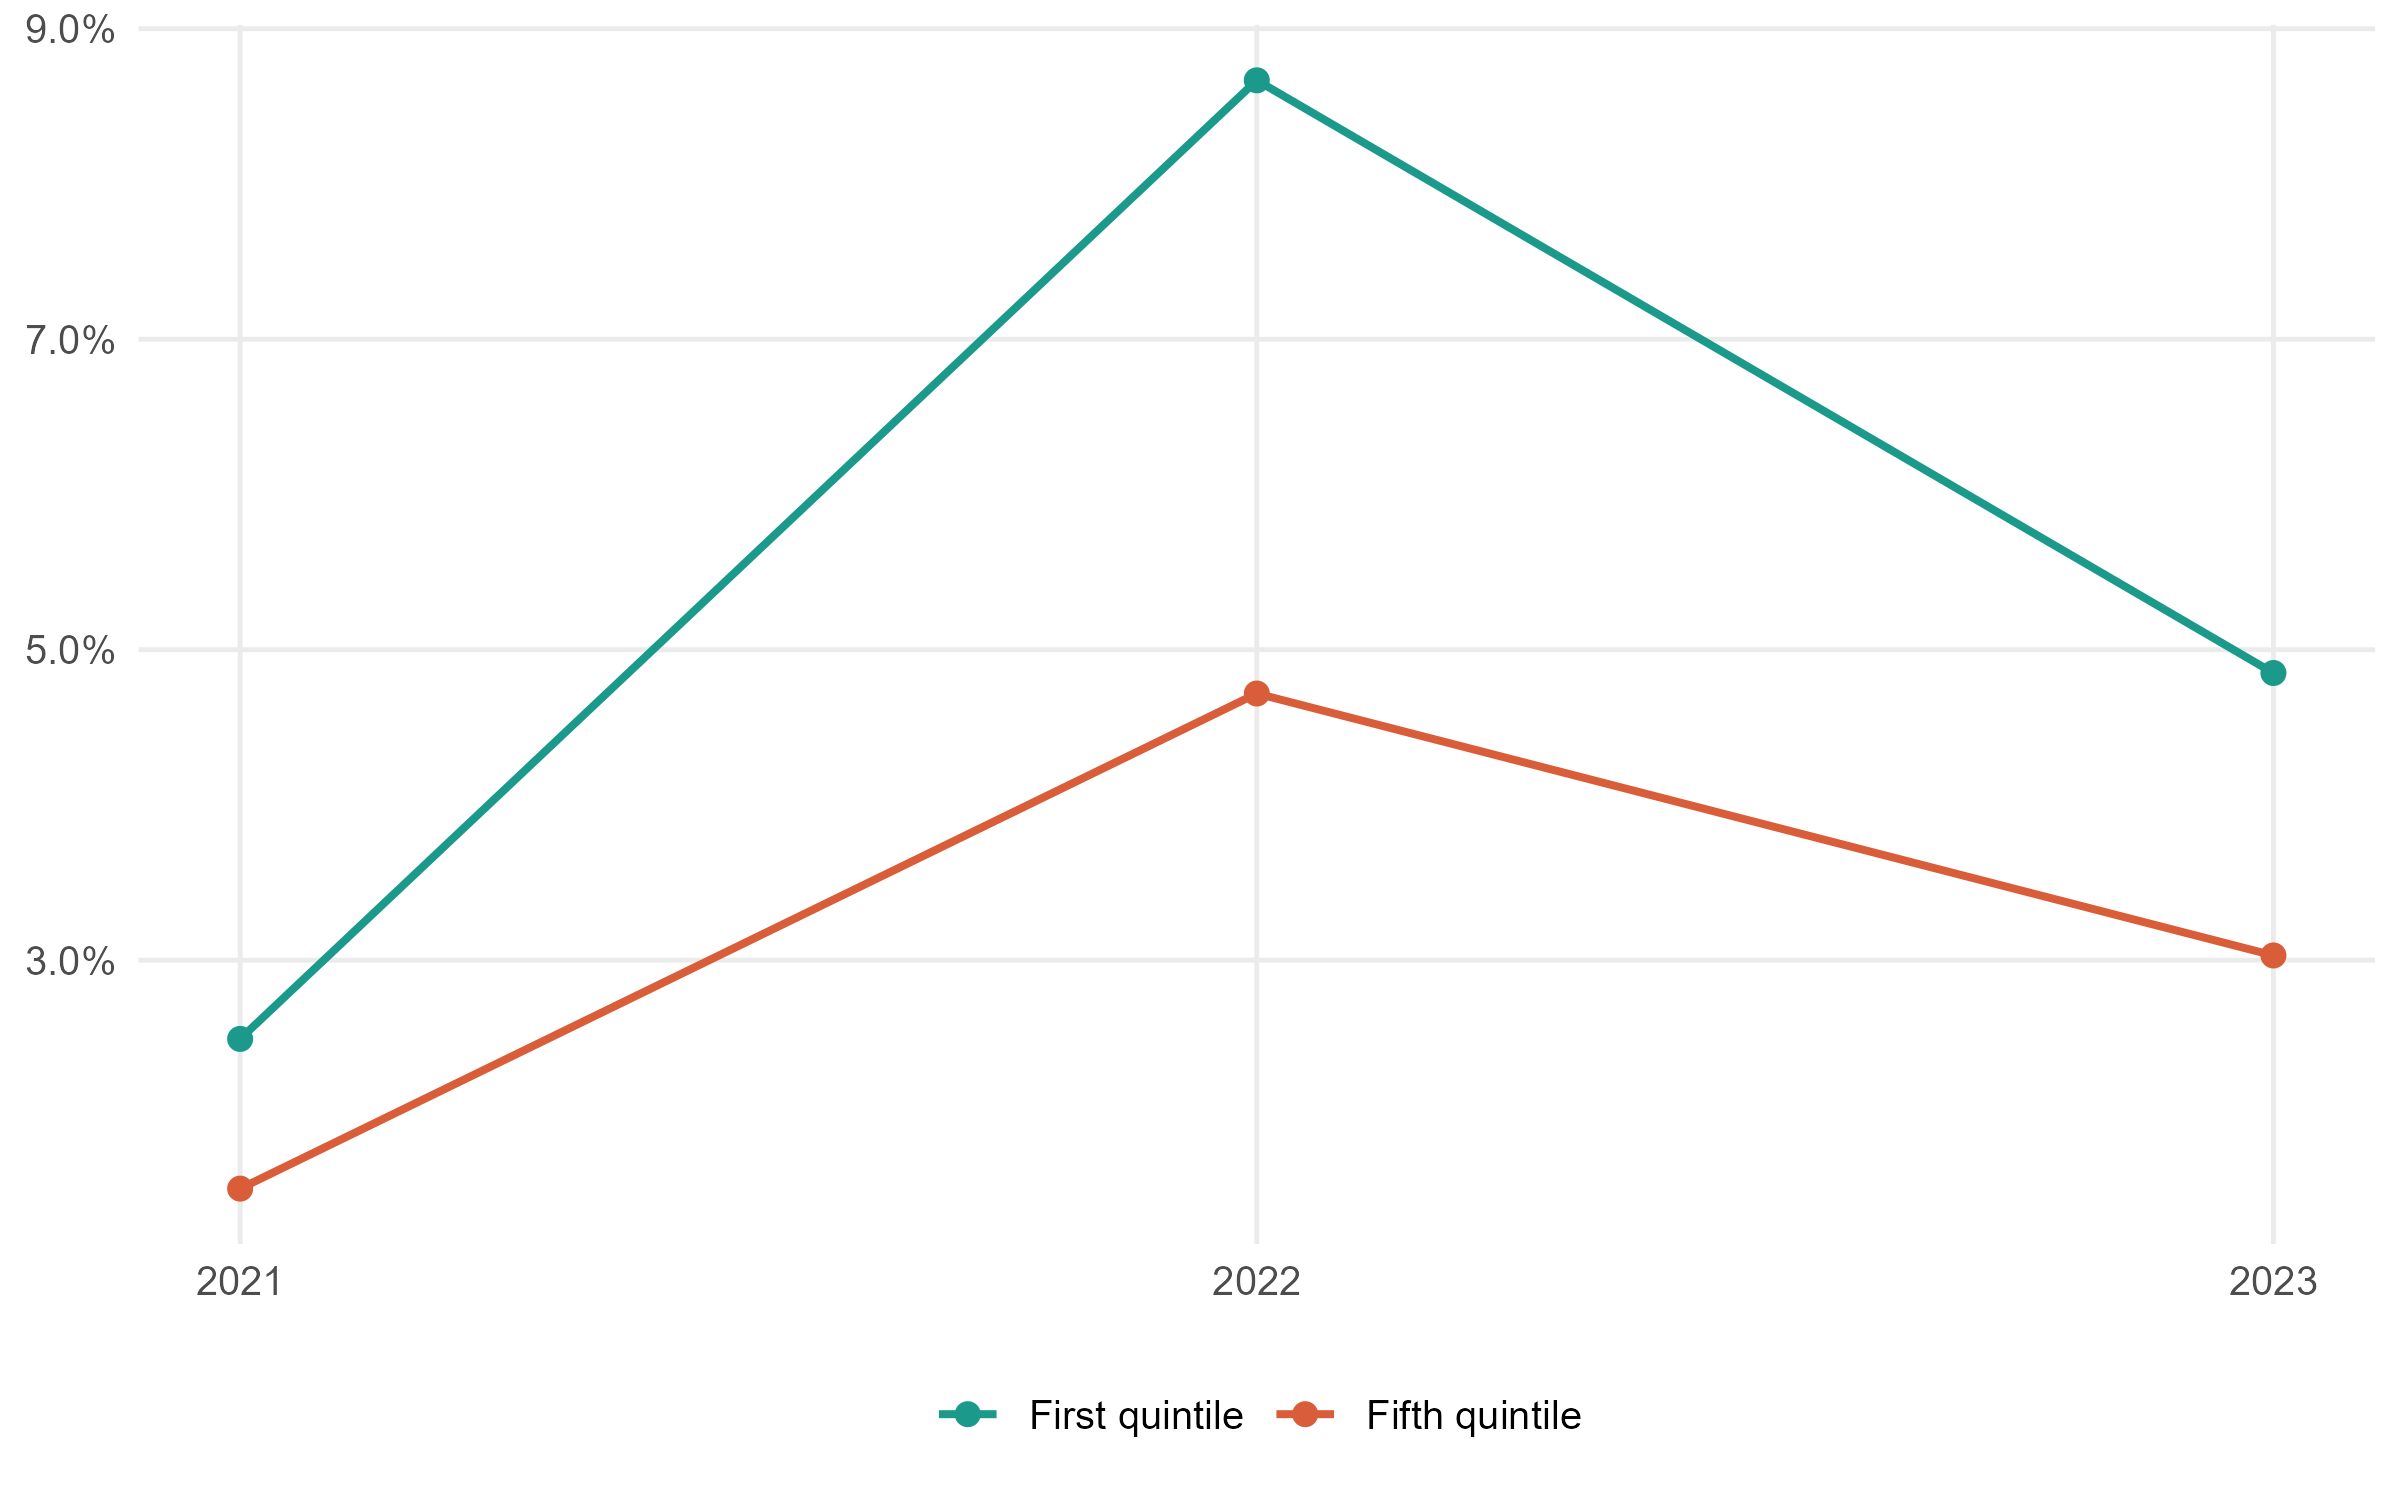
\includegraphics[width=0.95\textwidth,keepaspectratio]{fig_EA20_2019_2026_income_inflation_burden_Q1_Q5.png}
\vspace{4pt}
\captionsetup{font=footnotesize,format=hang,singlelinecheck=false,justification=justified}
\caption*{Notes: Annual household inflation times matched non-rent expenditure divided by net
income; ratios are winsorized at the national survey-weighted 99th percentile. Survey-weighted means
within national total-income quintiles, 18 countries excluding Italy and Portugal. Fixed 2020
resources; this is an exposure measure, not a welfare estimate.\\
Sources: HBS microdata, Eurostat HICP, authors' calculations.}
\end{figure}

\end{document}
